% ============================================================
% Question Bank: ch06-03 Drawing Geometric Figures with Given Conditions
% Topic Title: Drawing Geometric Figures with Given Conditions
% CCSS: 7.G.A.2
% Questions: 27 (15 MC + 6 SA + 6 Graphical)
% ============================================================

% --- Multiple Choice Questions (15) ---

\begin{practiceQuestion}{6-3-q01}{mc}
\begin{questionText}
Can you draw a triangle with sides $5$ cm, $7$ cm, and $13$ cm?
\end{questionText}
\choiceA{Yes, and it is a unique triangle}
\choiceB{Yes, and more than one triangle is possible}
\choiceC{No, because $5 + 7 < 13$}
\choiceD{No, because all three sides are odd numbers}
\correctAnswer{C}
\explanation{The triangle inequality requires the sum of any two sides to be greater than the third. Here $5 + 7 = 12 < 13$, so no triangle can be formed.}
\end{practiceQuestion}

\begin{practiceQuestion}{6-3-q02}{mc}
\begin{questionText}
Can you draw a triangle with sides $8$ cm, $8$ cm, and $8$ cm?
\end{questionText}
\choiceA{No, identical sides are not allowed}
\choiceB{Yes, exactly one equilateral triangle}
\choiceC{Yes, exactly two triangles}
\choiceD{Yes, infinitely many triangles}
\correctAnswer{B}
\explanation{All three inequality checks pass ($8 + 8 = 16 > 8$). Three equal sides (SSS) produce exactly one equilateral triangle.}
\end{practiceQuestion}

\begin{practiceQuestion}{6-3-q03}{mc}
\begin{questionText}
A quadrilateral has side lengths $5$, $5$, $5$, and $5$. How many different quadrilaterals can be drawn?
\end{questionText}
\choiceA{Exactly one (a square)}
\choiceB{Exactly two}
\choiceC{More than one}
\choiceD{None}
\correctAnswer{C}
\explanation{Four equal sides can form a square, a rhombus at any angle, or other shapes. The angles are not fixed, so many quadrilaterals are possible.}
\end{practiceQuestion}

\begin{practiceQuestion}{6-3-q04}{mc}
\begin{questionText}
You know two sides of a triangle are $9$ cm and $12$ cm, and the included angle is $60°$. How many different triangles can you draw?
\end{questionText}
\choiceA{None}
\choiceB{Exactly one}
\choiceC{Exactly two}
\choiceD{Infinitely many}
\correctAnswer{B}
\explanation{Two sides and the included angle (SAS) fully determine one unique triangle.}
\end{practiceQuestion}

\begin{practiceQuestion}{6-3-q05}{mc}
\begin{questionText}
Can a triangle have sides $10$, $10$, and $20$?
\end{questionText}
\choiceA{Yes, it is an isosceles triangle}
\choiceB{Yes, it is a right triangle}
\choiceC{No, the triangle inequality is not satisfied}
\choiceD{No, because two sides are equal}
\correctAnswer{C}
\explanation{$10 + 10 = 20$, which is not strictly greater than $20$. The triangle inequality requires a strict inequality, so no triangle can be formed.}
\end{practiceQuestion}

\begin{practiceQuestion}{6-3-q06}{mc}
\begin{questionText}
You know all three angles of a triangle: $30°$, $60°$, and $90°$. How many triangles can be drawn?
\end{questionText}
\choiceA{None}
\choiceB{Exactly one}
\choiceC{Exactly three}
\choiceD{Infinitely many}
\correctAnswer{D}
\explanation{Three angles (AAA) determine the shape but not the size. Infinitely many similar $30$-$60$-$90$ triangles of different sizes can be drawn.}
\end{practiceQuestion}

\begin{practiceQuestion}{6-3-q07}{mc}
\begin{questionText}
A rectangle must have an area of $36$ cm$^2$ with whole-number sides. How many different rectangles satisfy this condition?
\end{questionText}
\choiceA{$1$}
\choiceB{$4$}
\choiceC{$5$}
\choiceD{$9$}
\correctAnswer{C}
\explanation{Factor pairs of $36$: $1 \times 36$, $2 \times 18$, $3 \times 12$, $4 \times 9$, $6 \times 6$. That is $5$ different rectangles.}
\end{practiceQuestion}

\begin{practiceQuestion}{6-3-q08}{mc}
\begin{questionText}
Which set of conditions produces exactly one triangle?
\end{questionText}
\choiceA{Three angles: $45°$, $55°$, $80°$}
\choiceB{Two sides: $6$ cm and $10$ cm}
\choiceC{Two sides $5$ cm, $9$ cm and the included angle $40°$}
\choiceD{One side: $7$ cm}
\correctAnswer{C}
\explanation{SAS (two sides and the included angle) produces exactly one unique triangle. AAA gives many, and knowing only one or two sides without an angle is not enough.}
\end{practiceQuestion}

\begin{practiceQuestion}{6-3-q09}{mc}
\begin{questionText}
Can a triangle have sides $3$, $4$, and $3$?
\end{questionText}
\choiceA{No, two sides are equal}
\choiceB{No, the triangle inequality fails}
\choiceC{Yes, exactly one isosceles triangle}
\choiceD{Yes, infinitely many triangles}
\correctAnswer{C}
\explanation{Check: $3 + 3 = 6 > 4$, $3 + 4 = 7 > 3$, $3 + 4 = 7 > 3$. All pass. SSS gives exactly one unique isosceles triangle.}
\end{practiceQuestion}

\begin{practiceQuestion}{6-3-q10}{mc}
\begin{questionText}
A rhombus must have sides of $7$ cm. How many different rhombuses satisfy this condition?
\end{questionText}
\choiceA{None}
\choiceB{Exactly one}
\choiceC{Exactly four}
\choiceD{More than one}
\correctAnswer{D}
\explanation{A rhombus with sides of $7$ cm can have different angles. It could be a square or any slanted diamond shape. Many rhombuses are possible.}
\end{practiceQuestion}

\begin{practiceQuestion}{6-3-q11}{mc}
\begin{questionText}
Which set of side lengths can form a triangle?
\end{questionText}
\choiceA{$2$, $4$, $7$}
\choiceB{$4$, $5$, $10$}
\choiceC{$6$, $8$, $13$}
\choiceD{$1$, $3$, $5$}
\correctAnswer{C}
\explanation{Check: $6 + 8 = 14 > 13$ \checkmark, $6 + 13 = 19 > 8$ \checkmark, $8 + 13 = 21 > 6$ \checkmark. All other options fail the triangle inequality.}
\end{practiceQuestion}

\begin{practiceQuestion}{6-3-q12}{mc}
\begin{questionText}
Two angles of a triangle are $45°$ and $90°$. You also know the hypotenuse is $12$ cm. How many triangles can be drawn?
\end{questionText}
\choiceA{None}
\choiceB{Exactly one}
\choiceC{Exactly two}
\choiceD{Infinitely many}
\correctAnswer{B}
\explanation{The third angle is $180° - 45° - 90° = 45°$. Two angles and a specific side (AAS) determine exactly one triangle.}
\end{practiceQuestion}

\begin{practiceQuestion}{6-3-q13}{mc}
\begin{questionText}
Amir wants to draw a triangle with angles $60°$, $70°$, and $50°$ and one side of $10$ cm. How many triangles can he draw?
\end{questionText}
\choiceA{None}
\choiceB{Exactly one}
\choiceC{Exactly three}
\choiceD{Infinitely many}
\correctAnswer{C}
\explanation{With three angles and one side, the position of the known side matters. It could be opposite any of the three angles, giving up to $3$ triangles of different sizes. Each placement determines a unique triangle.}
\end{practiceQuestion}

\begin{practiceQuestion}{6-3-q14}{mc}
\begin{questionText}
Which condition makes it impossible to draw a triangle?
\end{questionText}
\choiceA{Sides $7$, $10$, $12$}
\choiceB{Sides $3$, $5$, $3$}
\choiceC{Sides $4$, $4$, $9$}
\choiceD{Sides $6$, $6$, $6$}
\correctAnswer{C}
\explanation{$4 + 4 = 8 < 9$. The triangle inequality fails. The other sets all satisfy the triangle inequality.}
\end{practiceQuestion}

\begin{practiceQuestion}{6-3-q15}{mc}
\begin{questionText}
Which set of conditions produces more than one possible triangle?
\end{questionText}
\choiceA{Sides $4$, $7$, $9$ (SSS)}
\choiceB{Sides $6$ and $10$ with included angle $50°$ (SAS)}
\choiceC{Angles $35°$, $65°$, $80°$ (AAA)}
\choiceD{Angles $40°$, $50°$ with included side $8$ cm (ASA)}
\correctAnswer{C}
\explanation{AAA determines the shape but not the size. Many similar triangles of different sizes can have these angles. SSS, SAS, and ASA each produce exactly one triangle.}
\end{practiceQuestion}

% --- Short Answer Questions (6) ---

\begin{practiceQuestion}{6-3-q16}{sa}
\begin{questionText}
Can a triangle have sides $12$ cm, $5$ cm, and $4$ cm? Explain why or why not.
\end{questionText}
\correctAnswer{No}
\explanation{$5 + 4 = 9 < 12$. The sum of the two shorter sides is less than the longest side. The triangle inequality is not satisfied.}
\end{practiceQuestion}

\begin{practiceQuestion}{6-3-q17}{sa}
\begin{questionText}
A triangle has two sides of length $6$ cm and $14$ cm. What is the range of possible lengths for the third side?
\end{questionText}
\correctAnswer{Greater than $8$ cm and less than $20$ cm}
\explanation{By the triangle inequality: $14 - 6 < \text{third side} < 14 + 6$, so $8 < \text{third side} < 20$.}
\end{practiceQuestion}

\begin{practiceQuestion}{6-3-q18}{sa}
\begin{questionText}
A triangle has sides $8$, $15$, and $17$. What type of triangle is it?
\end{questionText}
\correctAnswer{Right triangle}
\explanation{Check: $8^2 + 15^2 = 64 + 225 = 289 = 17^2$. The Pythagorean theorem holds, so it is a right triangle.}
\end{practiceQuestion}

\begin{practiceQuestion}{6-3-q19}{sa}
\begin{questionText}
How many different rectangles have a perimeter of $28$ cm with whole-number sides?
\end{questionText}
\correctAnswer{$7$}
\explanation{Half-perimeter is $14$. Pairs: $1 \times 13$, $2 \times 12$, $3 \times 11$, $4 \times 10$, $5 \times 9$, $6 \times 8$, $7 \times 7$. That is $7$ different rectangles.}
\end{practiceQuestion}

\begin{practiceQuestion}{6-3-q20}{sa}
\begin{questionText}
A square has an area of $49$ cm$^2$. How many different squares satisfy this condition?
\end{questionText}
\correctAnswer{$1$}
\explanation{A square with area $49$ cm$^2$ has side $\sqrt{49} = 7$ cm. All squares with side $7$ cm are congruent, so exactly one square satisfies this.}
\end{practiceQuestion}

\begin{practiceQuestion}{6-3-q21}{sa}
\begin{questionText}
You know two angles of a triangle: $55°$ and $55°$. Is the triangle unique? Explain.
\end{questionText}
\correctAnswer{No, the triangle is not unique}
\explanation{The third angle is $180° - 55° - 55° = 70°$. Three angles (AAA) fix the shape but not the size. Many isosceles triangles with these angles exist.}
\end{practiceQuestion}

% --- Graphical MC Questions (3) ---

\begin{practiceQuestion}{6-3-q22}{gmc}
\begin{questionText}
Which of the following sets of side lengths can form the triangle shown below?

\begin{center}
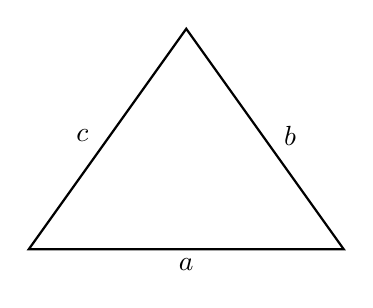
\begin{tikzpicture}[scale=0.8]
  \draw[thick] (0,0) -- (5,0) -- (2.5,3.5) -- cycle;
  \node[below] at (2.5,0) {$a$};
  \node[right] at (3.9,1.8) {$b$};
  \node[left] at (1.1,1.8) {$c$};
\end{tikzpicture}
\end{center}
\end{questionText}
\choiceA{$a = 2$, $b = 3$, $c = 6$}
\choiceB{$a = 5$, $b = 1$, $c = 3$}
\choiceC{$a = 7$, $b = 5$, $c = 4$}
\choiceD{$a = 1$, $b = 1$, $c = 3$}
\correctAnswer{C}
\explanation{Check: $7 + 5 = 12 > 4$, $7 + 4 = 11 > 5$, $5 + 4 = 9 > 7$. All triangle inequality checks pass. The other options fail.}
\end{practiceQuestion}

\begin{practiceQuestion}{6-3-q23}{gmc}
\begin{questionText}
The diagram below shows two sides and an included angle. How many triangles can be drawn with these measurements?

\begin{center}
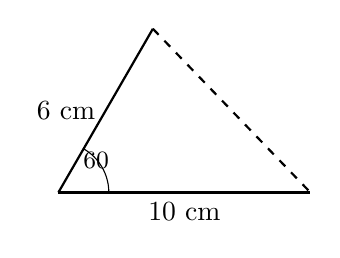
\begin{tikzpicture}[scale=0.8]
  \draw[thick] (0,0) -- (4,0) node[midway,below] {$10$ cm};
  \draw[thick] (0,0) -- (60:3) node[midway,left] {$6$ cm};
  \draw[thick,dashed] (60:3) -- (4,0);
  \draw (0.8,0) arc (0:60:0.8);
  \node at (0.6,0.5) {\small $60°$};
\end{tikzpicture}
\end{center}
\end{questionText}
\choiceA{None}
\choiceB{Exactly one}
\choiceC{Exactly two}
\choiceD{Infinitely many}
\correctAnswer{B}
\explanation{Two sides ($6$ cm and $10$ cm) and the included angle ($60°$) is SAS. This produces exactly one unique triangle.}
\end{practiceQuestion}

\begin{practiceQuestion}{6-3-q24}{gmc}
\begin{questionText}
The polygon below has four sides with the lengths shown. How many different quadrilaterals can be drawn with these side lengths?

\begin{center}
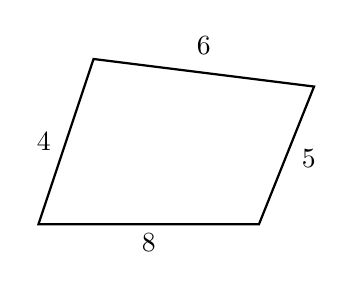
\begin{tikzpicture}[scale=0.7]
  \draw[thick] (0,0) -- (4,0) -- (5,2.5) -- (1,3) -- cycle;
  \node[below] at (2,0) {$8$};
  \node[right] at (4.6,1.2) {$5$};
  \node[above] at (3,2.9) {$6$};
  \node[left] at (0.4,1.5) {$4$};
\end{tikzpicture}
\end{center}
\end{questionText}
\choiceA{Exactly one}
\choiceB{Exactly two}
\choiceC{More than one}
\choiceD{None}
\correctAnswer{C}
\explanation{Four side lengths alone do not fix the angles of a quadrilateral. The shape can be pushed and pulled into many configurations, so more than one quadrilateral is possible.}
\end{practiceQuestion}

% --- Graphical SA Questions (3) ---

\begin{practiceQuestion}{6-3-q25}{gsa}
\begin{questionText}
The triangle below has angles $50°$, $60°$, and $70°$. Is this the only triangle with these angles, or can others exist? Explain.

\begin{center}
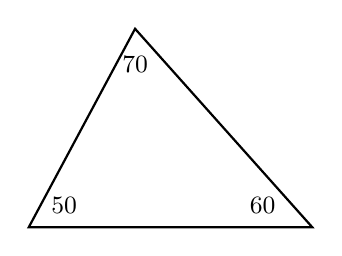
\begin{tikzpicture}[scale=0.9]
  \draw[thick] (0,0) -- (4,0) -- (1.5,2.8) -- cycle;
  \node at (0.5,0.3) {\small $50°$};
  \node at (3.3,0.3) {\small $60°$};
  \node at (1.5,2.3) {\small $70°$};
\end{tikzpicture}
\end{center}
\end{questionText}
\correctAnswer{Others exist; infinitely many similar triangles can share these angles}
\explanation{AAA (three angles) determines the shape but not the size. Many triangles of different sizes can have angles $50°$, $60°$, and $70°$.}
\end{practiceQuestion}

\begin{practiceQuestion}{6-3-q26}{gsa}
\begin{questionText}
A student tries to build a triangle with the side lengths shown below. Is the triangle possible? If so, state whether it is unique.

\begin{center}
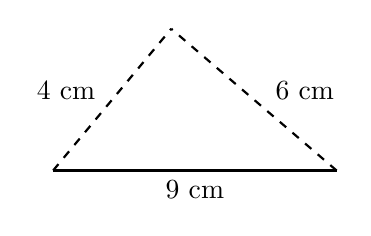
\begin{tikzpicture}[scale=0.6]
  \draw[thick] (0,0) -- (6,0);
  \draw[thick,dashed] (0,0) -- (2.5,3);
  \draw[thick,dashed] (6,0) -- (2.5,3);
  \node[below] at (3,0) {$9$ cm};
  \node[left] at (1.1,1.7) {$4$ cm};
  \node[right] at (4.5,1.7) {$6$ cm};
\end{tikzpicture}
\end{center}
\end{questionText}
\correctAnswer{Yes, exactly one triangle}
\explanation{Check the triangle inequality: $4 + 6 = 10 > 9$, $4 + 9 = 13 > 6$, $6 + 9 = 15 > 4$. All pass, so a triangle can be formed. SSS produces exactly one unique triangle.}
\end{practiceQuestion}

\begin{practiceQuestion}{6-3-q27}{gsa}
\begin{questionText}
The figure shows a triangle with two given angles. Find the value of the missing angle and state whether the triangle is unique.

\begin{center}
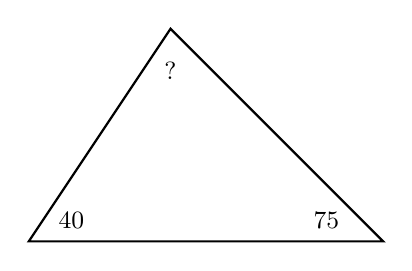
\begin{tikzpicture}[scale=0.9]
  \draw[thick] (0,0) -- (5,0) -- (2,3) -- cycle;
  \node at (0.6,0.3) {\small $40°$};
  \node at (4.2,0.3) {\small $75°$};
  \node at (2,2.4) {\small $?$};
\end{tikzpicture}
\end{center}
\end{questionText}
\correctAnswer{$65°$; the triangle is not unique (infinitely many sizes)}
\explanation{The missing angle is $180° - 40° - 75° = 65°$. Three angles (AAA) fix the shape but not the size, so the triangle is not unique.}
\end{practiceQuestion}
